\chapter{Learning from Limited Supervised Data I: Using Unlabelled Videos}
\label{chap:limited}
Previously, we have developed \gbcnet to tackle the issues in USG images and achieved superior GBC detection performance compared to the state-of-the-art CNN models, and expert radiologists. However, the reliance on bounding box annotations to train the ROI detection phase in \gbcnet poses a bottleneck. Medical data annotation requires trained medical experts. The cost of obtaining annotations is thus very high due to the complexity and involvement of trained experts. Such annotation also adds additional burden on the medical professionals as they already face time constraints due to high patient influx. In this chapter, we tackle a key challenge associated with medical image computing and analysis -- paucity of annotated dataset, and explore the utilization of limited supervised data for training deep neural networks (DNNs) to detect GBC from USG images. In this chapter, 
%We investigate two distinct approaches towards this direction -- (1) 
we introduce an unsupervised contrastive framework designed to leverage unlabelled video data for effective representation learning, ultimately benefiting downstream GBC detection from USG images.%, and (2) we use a weakly supervised object detection technique to detect GBC with only image-level labels instead of the costly bounding box annotations during training. 
The contents in this chapter are based on the following published work:
\par \noindent [1] \textit{Soumen Basu, Somanshu Singla, Mayank Gupta, Pratyaksha Rana, Pankaj Gupta, and Chetan Arora.
``Unsupervised Contrastive Learning of Image Representations from Ultrasound Videos with Hard Negative Mining.'' International Conference on Medical Image Computing and Computer-Assisted Intervention (MICCAI). 2022}. 

%\section{Representation Learning with Unlabelled Video Data}
\label{chap:usucl}

%Rich temporal information and variations in viewpoints make video data an attractive choice for learning image representations using unsupervised contrastive learning (UCL) techniques. State-of-the-art (SOTA) contrastive learning techniques consider frames within a video as positives in the embedding space, whereas the frames from other videos are considered negatives. We observe that unlike multiple views of an object in natural scene videos, an USG video captures different 2D slices of an organ. Hence, there is almost no similarity between the temporally distant frames of even the same USG video. In this paper we propose to instead utilize such frames as hard negatives. We advocate mining both intra-video and cross-video negatives in a hardness-sensitive negative mining curriculum in a UCL framework to learn rich image representations. We deploy our framework to learn the representations of Gallbladder (GB) malignancy from USG videos. We also construct the first large-scale USG video dataset containing 64 videos and 15,800 frames for learning GB representations. We show that the standard ResNet50 backbone trained with our framework improves the accuracy of models pretrained with SOTA UCL techniques as well as supervised pretrained models on ImageNet for the GB malignancy detection task by 2--6\%. We further validate the generalizability of our method on a publicly available lung USG image dataset of COVID-19 pathologies and show an improvement of 1.5\% compared to SOTA. Source code, dataset, and models are available at \url{https://gbc-iitd.github.io/usucl}.
	
% \keywords{Contrastive Learning \and Ultrasound \and Negative Mining}
% \end{abstract}

% ---- Introduction ----
%
\section{Introduction}

%Due to their remarkable performance, Deep Neural Networks (DNNs) have become defacto standard for a wide range of medical image analysis tasks in recent years \cite{ardila2019end,bejnordi2017diagnostic}. However, 
Lack of annotated medical data due to the specialized nature of annotations, and the data privacy issues restrict the applicability of supervised learning of DNNs in medical imaging. Although pretraining on large natural image datasets yields a performance boost for downstream tasks on medical data \cite{alzubaidi2020transferlearning,cheng2017transfer}, the large domain gap between the natural and medical images remains a bottleneck. Recent works are increasingly going beyond the supervised setup and exploiting unsupervised techniques to compensate for the lack of annotated data \cite{simclr,moco}. Broadly, there are two prominent categories of representation learning techniques for leveraging unlabeled data. In the pretext task-based method, the DNNs are pretrained with some spatial tasks such as image rotation prediction \cite{komodakis2018unsupervised} or temporal tasks such as video clip order prediction \cite{xu2019self} to learn efficient image representation. On the other hand, contrastive methods \cite{simclr} try to distinguish between different views of image samples to learn robust representation without labels. Visual representations learned by contrastive learning have been shown to outperform the supervised pretraining on large annotated data in terms of accuracy on the downstream prediction tasks \cite{simclr,moco}.  

\begin{figure}[t]
    \centering
    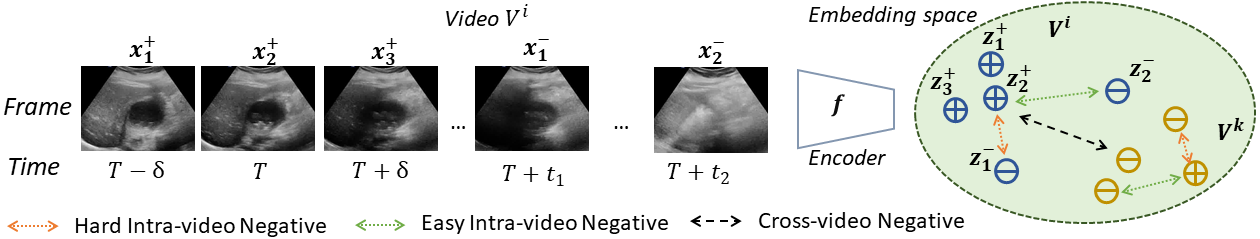
\includegraphics[width=\linewidth]{figs/usucl/teaser.png}
    \caption[Motivation of using intra-video negatives]{We motivate the use of intra-video negatives in contrastive learning. Based on the visibility of a pathology in the intra-video samples, negatives can be sampled. The frames in range $[T-\delta, T+\delta]$ in video $V^i$ has stones and malignant wall thickening visible for a small $\delta$. A slightly distant frame $T+t_1$ shows a GB, but the malignant wall thickening is not visible. This sample acts as a hard negative. The viewing plane further changes in frame $T+t_2$ and GB becomes invisible.}
    \label{usucl_fig:teaser}
\end{figure}

Video data contains rich variations in viewpoints and natural temporal information for objects making it suitable for going beyond image-level contrastive learning. Additionally, the abundance of unlabeled video data makes it an attractive choice for learning representations. Recent works are attempting to exploit the video data to learn robust image-level representations \cite{uscl,cyclecontrast}. We observe that current SOTA techniques for image representation learning from videos, such as USCL \cite{uscl} suggest that images coming from the same video are too close to be considered negatives (\emph{similarity conflict}). USCL advocates considering only cross-video samples as negatives to avoid the similarity conflict. While similarity conflict is prevalent for intra-video samples of natural video datasets like action recognition, where each video contains a distinct action, the USG videos are inherently different. We observe that unlike multiple views of an object in natural scene videos, an USG video captures different 2D slices of an organ. Hence, there is almost no similarity between the temporally distant frames of even the same USG video. We propose to instead utilize such frames as negatives. The frames of a USG video contain both types of images where pathology maybe visible or absent. \cref{usucl_fig:teaser} shows the positive and negative frames from the same USG video. The temporal distance between the frames acts as a proxy to the hardness. Negative samples that are temporally closer to the positives contain higher similarities with the positives and are harder to differentiate in the embedding space. We propose an unsupervised contrastive framework to exploit both the intra-video and cross-video negatives for learning robust visual representations from USG videos. We design a hardness-sensitive negative mining curriculum to lower the distance between the anchor and negatives gradually. Due to its unsupervised nature, our technique can be used for pretraining a backbone on any USG video dataset for superior downstream performance.

We deploy our video contrastive learning framework to pretrain a neural network before supervised fine-tuning to identify GBC in USG images. 
%Due to its non-ionizing radiation, low cost, and accessibility, USG is a popular non-invasive diagnostic modality for patients with suspected GB pathology. Although there are prior works involving DNNs to detect GB afflictions such as polyp or stones \cite{gbPolyp,gbPolyp2,gbAutomatic}, there is limited prior work on using DNNs to detect GB malignancy in USG images \cite{basu2022surpassing}. 
Unlike detecting stones or polyps, identifying GB malignancy from the routine USG is challenging for radiologists \cite{gb-rads-paper,gupta2020imaging}. We observed that ImageNet pretrained classifiers perform even worse than radiologists. 
%We used an USG video dataset to pretrain our model. 
Our contrastive learning-based pretraining on USG videos help the model to surpass human radiologists and SOTA contrastive learning methods on GBC classification.

We also validate the generality our framework on a public lung USG dataset, POCUS \cite{pocus}, containing COVID-19 and Pneumonia samples. Pretraining our model on public lung USG videos, and finetuning for the downstream classification shows improvement over ImageNet pretraining and the current SOTA contrastive techniques.

% \mypara{Contributions} Our key contributions in this chapter are:
% \begin{itemize}
% \itemsep0em
% 	\item  We design an unsupervised contrastive learning technique for USG videos to exploit both cross-video and intra-video negatives for rich representation learning. We further use a hardness-sensitive negative mining curriculum to boost the performance of our contrastive learning framework.
% 	%
% 	\item We deploy our framework to solve a novel GB malignancy classification problem from USG images. We also validate the efficacy of our technique on a publicly available lung USG dataset for COVID detection.
% 	%
% 	%\item We are contributing the first USG video dataset of 64 videos and 15800 frames containing both malignant and non-malignant GB towards the development of representation learning from medical USG videos.
% \end{itemize}

% ---- Dataset ----
%
\begin{figure}[t]
    \centering
    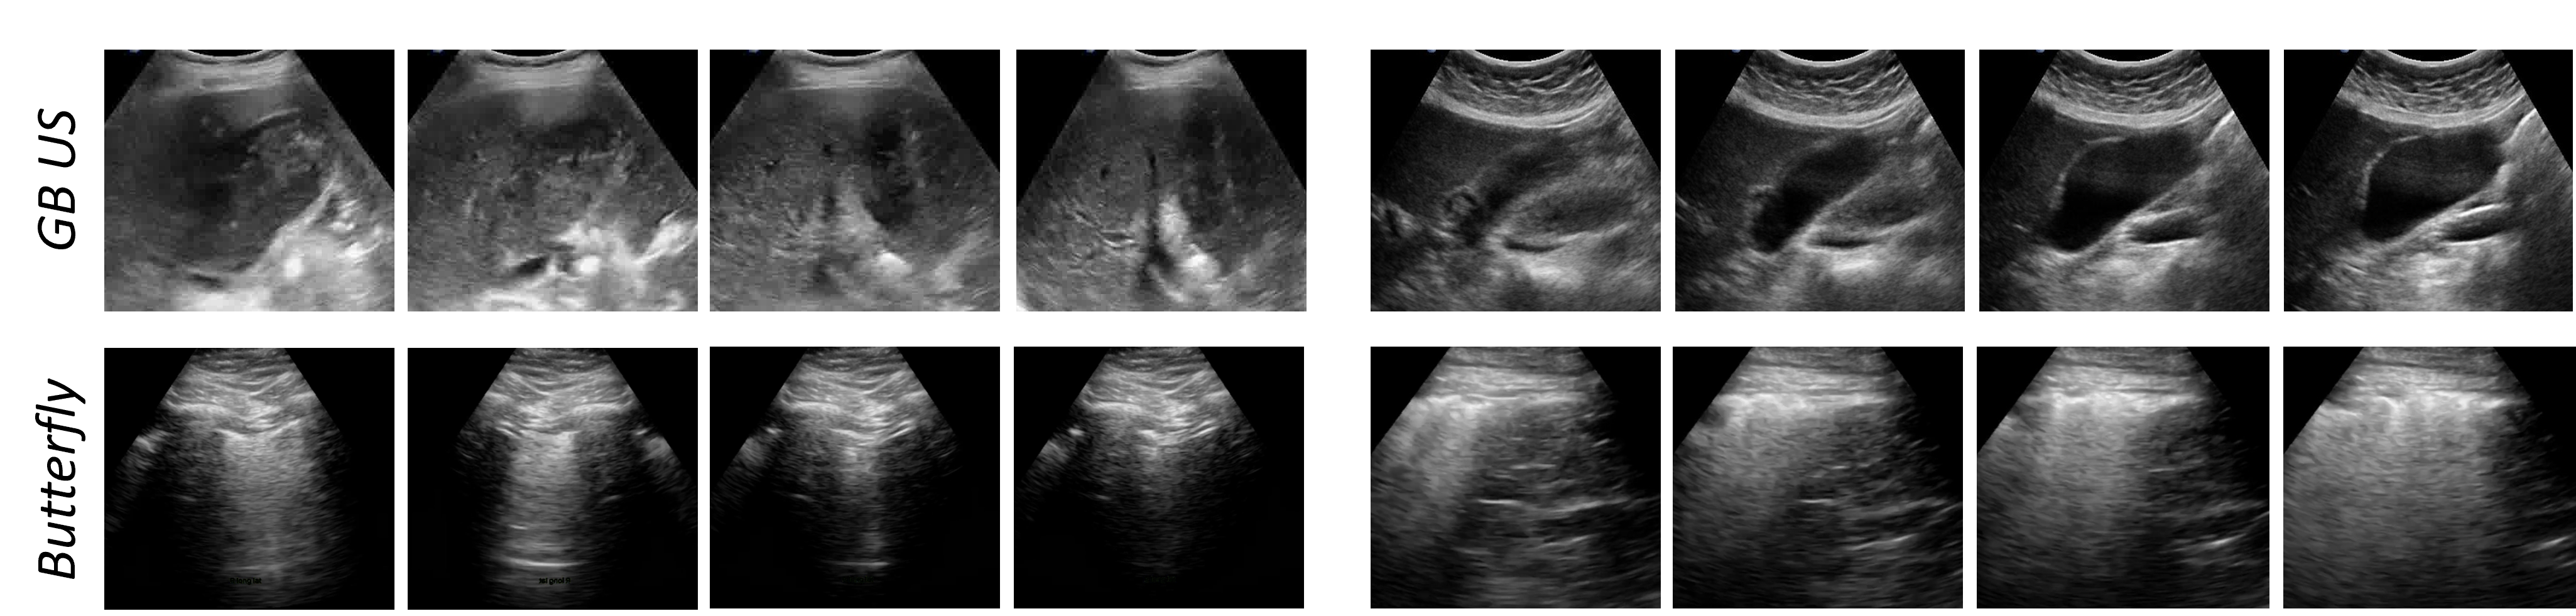
\includegraphics[width=0.9\linewidth]{figs/usucl/data_sample.png}
    \caption[Sample video sequences for the GBC and Covid Ultrasound data]{Sample video sequences from the GB USG video and the Butterfly \cite{butterfly} datasets. Two sequences of size 4 is shown on the left and right for each dataset.}
    \label{usucl_fig:data_sample}
\end{figure}
%
\section{Data}
%
\subsection{USG Dataset for Gallbladder Cancer}
%
We have used the GBUSV dataset described in \cref{data:gbusv} for the unsupervised contrastive pretraining, and the GBCU dataset (\cref{data:gbcu}) for the downstream GBC classification task. For helping the reader, we briefly describe the data in this section as well.

\mypara{Video Data for Contrastive Pretraining}
%
Radiologists with 2-8 years of experience in abdominal sonography acquired the data. The USG videos were obtained after at least 6 hours of fasting using a 1--5 MHz curved array transducer (C-1-5D, Logiq S8, GE Healthcare). The scanning intended to include the entire GB and the lesion or pathology. %The frame rate was 29 fps. 
The length of the videos varied from 43 to 888 frames. %depending on the GB distension and size of the lesion. 
The dataset consists of 32 malignant and 32 non-malignant videos containing a total of 12,251 and 3,549 frames, respectively. We do not use the video level labels in the contrastive pretraining. We cropped the video frames from the center to anonymize the patient information. The processed video frames were of size $360\!\times\!480$ pixels. \cref{usucl_fig:data_sample} shows some samples from the video data. 

\mypara{Image Data for Downstream GBC Classification}
%
GBCU dataset \cite{basu2022surpassing} consists of 1255 USG images from 218 patients. The images were labeled as normal, benign, or malignant, and such labels were biopsy-proven. The dataset consists of 990 non-malignant (432 normal, 558 benign) and 265 malignant images.  We use this dataset for finetuning and report 10-fold cross-validation. We did the cross-validation splits at the patient level. 
The patients recorded in the video dataset are different from the patients used in the image dataset to ensure generalization. 

\subsection{Public Lung USG Dataset for COVID-19}

\myfirstpara{Video Data}
%
We use the public lung USG video dataset, Butterfly \cite{butterfly}. Butterfly consists of 22 USG videos containing 1533 images of size $658\!\times\!758$ pixels of the lung. The dataset was collected using a Resona 7T machine.

\mypara{Image Data}
%
We use the publicly available POCUS \cite{pocus} dataset consisting of a total of 2116 lung USG images, of which 655, 349, and 1112 images are of COVID-19, bacterial pneumonia, and healthy control, respectively.

%
% ---- Methods ----
%
\section{Methodology}

\begin{figure}[t]
    \centering
    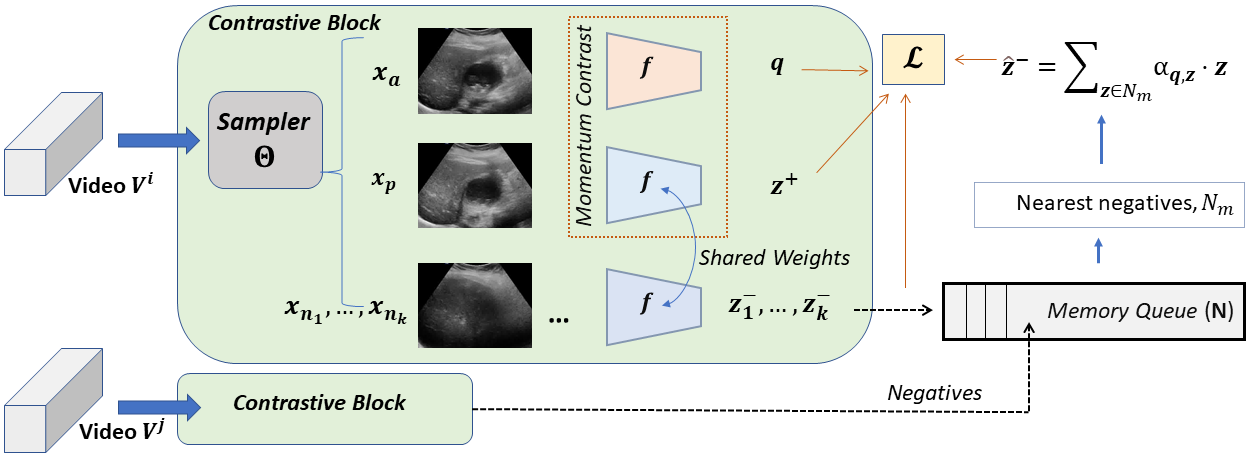
\includegraphics[width=0.9\linewidth]{figs/usucl/arch1.png}
    \caption[Overview of the proposed contrastive framework]{Overview of the proposed contrastive loss, $\mathcal{L}$. An anchor $\vb{q}$ and another temporally close sample $\vb{z}^+$ from the same video are used as positive pairs. Given the set of cross-video negatives $N$, and the intra-video negatives $\vb{z}_j^-$, we compute $\vb{\hat{z}}^-$ from the $m$ most similar cross-video negatives to the anchor. The intra-video samples $\vb{z}_j^-$ and $\vb{\hat{z}}^-$ are considered as negatives to the anchor.}
    \label{usucl_fig:my_label}
\end{figure}

\mypara{Contrastive Learning Setup}
%
Suppose, $\vb{V}^i = \big\{ \vb{x}_j\big\}_{j=1}^{M^i}$ is the $i$-th video in the video dataset consisting of $M^i$ frames where $\vb{x}_j$ is the $j$-th individual frame. We sample an anchor image, $\vb{x}_a$, a positive image $\vb{x}_p$, and $k$ negative frames $\vb{x}_{n_1}, \ldots, \vb{x}_{n_k}$ from a video using a sampler $\vb{\Theta}$. We encode the samples using a backbone $f$ followed by a two layer MLP, $g$ that creates a 128 dimensional embedding vector. We denote the embedding vectors as:
%
\begin{align}
    \vb{q} = g(f(\vb{x}_a)), \qquad
    \vb{z}^+ = g(f(\vb{x}_p)), ~ \text{and} \qquad
    \vb{z}_j^- = g(f(\vb{x}_{n_j})).
\end{align}
%
We maximize the agreement between (positive, anchor) and minimize between (anchor, negatives) pairs in the embedding space. Let $N$ be the set of cross video negatives generated from other videos in the dataset. To exploit the cross-video negatives, we calculate the normalized similarity measure between $\vb{q}$ and $\vb{z}$ for all $\vb{z} \in N$:
%
\begin{align}
    \alpha_{\vb{q},\vb{z}}= \frac{\exp\big(s(\vb{q}, \vb{z})/\tau\big)}{ \sum_{\vb{z}_c\in N}\exp\big(s(\vb{q}, \vb{z}_c)/\tau\big)},
\end{align}
%
where $s(\vb{a}, \vb{b}) = \vb{a}\cdot \vb{b}\big/(||\vb{a}||_2~ ||\vb{b}||_2)$ is the cosine similarity and $\tau$ is a temperature scaling parameter.
We then use the $\alpha_{\vb{q},\vb{z}}$ to rank the cross-video negatives according to their similarity with the anchor. Note that, with increasing similarity, the hardness of the negatives increase. We pick the top-$n$ hardest cross-video negatives, $N_m$, and compute $\vb{\hat{z}}^- = \sum_{\vb{z}\in N_m}{\alpha_{\vb{q},\vb{z}} \vb{z}}$. 
Finally, we minimize the loss,
%
\begin{align}
    \mathcal{L} = -\log \frac{\exp\big(s(\vb{q}, \vb{z}^+)/\tau\big)}{\exp\big(s(\vb{q}, \vb{z}^+)/\tau\big) + \sum_{j=1}^k\exp\big(s(\vb{q}, \vb{z}_j^-)/\tau\big) + \exp\big(s(\vb{q}, \vb{\hat{z}}^-)/\tau\big)}.
\label{eqn:loss_term}
\end{align}
%
Note that $\vb{z}_j^-$ is obtained intra-video, and $\vb{\hat{z}}^-$ is obtained from inter-video samples. Hence, $\mathcal{L}$ exploits both the intra-video and cross-video hard negatives. We chose $\tau\!=\!0.07$. Value of $n$ was $4$ and $2$ for GB videos and Butterfly, respectively.

\mypara{Video Sub-Sampling}
%
Most SOTA methods sample the anchor and positive pairs uniformly at random from the entire sequence of frames in a video. However, in the case of USG videos, the view may change significantly if the samples are temporally distant. For example, in a transabdominal USG video, one sample may show a GB with some parts of a liver while another may show only a liver and not a GB. Pairing such samples as positives would not work for learning a representation of the GB pathology. We recommend sampling the anchor and positives from a temporally close interval. We use a sampler, $\vb{\Theta}\!:\!\vb{V}\!\rightarrow\!\big(\vb{x}_a, \vb{x}_p, \{\vb{x}_{n_1}, \ldots, \vb{x}_{n_k}\}\big)$ to get the anchor ($\vb{x}_a$), positive ($\vb{x}_p$), and $k$ negative frames ($\vb{x}_{n_1}, \ldots, \vb{x}_{n_k}$) from a video $\vb{V}\!=\!\big\{ \vb{x}_j\big\}_{j=1}^M$. The indices of the anchor, positive, and negative frames are sampled as following: 
%
\begin{align*}
a \overset{\hphantom{\text{i.i.d.}}}{\sim} U\big([1,M]\big), 
\qquad
p \overset{\hphantom{\text{i.i.d.}}}{\sim} U\big([a-\delta, a+\delta] \setminus \{a\}\big), 
\\ 
n_1, \ldots, n_k \overset{\text{i.i.d.}}{\sim} U\big([1,M] \setminus [a-\Delta,a+\Delta]\big)
\label{eqn:neg_sample}
\end{align*} 
%
where $U(I)$ denotes sampling uniformly at random from interval $I$. We vary $\Delta$ between the $\Delta_h$ and $\Delta_l$ during the curriculum to adjust the hardness of the mined negatives. Also, $1 \le \delta \ll\ \!M$ and $ \Delta_{l} \le \Delta \le \Delta_{h} < M$. 

\mypara{Curriculum-based Negative Mining}
%
We use the negative samples in a hardness-sensitive order for effective learning. The model would initially learn to distinguish anchors from distant negatives and then gradually closer and thus harder negatives will be introduced. We start the training with only cross-video negatives and minimize the loss term, 
%
\begin{align}
    \mathcal{L}_{\text{cross}} = -\log \frac{\exp\big(s(\vb{q}, \vb{z}^+)/\tau\big)}{\exp\big(s(\vb{q}, \vb{z}^+)/\tau\big) + \exp\big(s(\vb{q}, \vb{\hat{z}}^-)/\tau\big)}.
\end{align}
We then gradually start using the loss in \cref{eqn:loss_term} to introduce intra-video negatives, which are more challenging to distinguish from the anchor than the cross-video negatives. We initially keep the $\Delta= \Delta_h =\lceil M/5\rceil$ used in \cref{eqn:neg_sample} for sampling the negatives and ensure the anchor and negatives are at least $\Delta$ frames apart temporally, and the hardness is comparatively lower. We gradually lower the $\Delta$ using a cosine annealing during the later phase of training to introduce harder negatives. We chose $\delta=3$, $k=3$, and  $\Delta_l=7$ in our experiments.

%
% ---- Experiments and Results ----
%
\begin{table}[t]
	\centering
    \footnotesize
	\setlength{\tabcolsep}{10pt}
    %\resizebox{ \linewidth}{!}{%
	\begin{tabular}{lccc}
		\toprule
		\textbf{Method}	& \textbf{Acc.} & \textbf{Spec.} & \textbf{Sens.} \\
		\midrule
		%
		Pretrained on ImageNet \cite{imagenet} & 0.867 $\pm$ 0.070 & 0.926 $\pm$ 0.069 & 0.672 $\pm$ 0.147 \\
		%
		\midrule
		%
		SimCLR \cite{simclr} & 0.897 $\pm$ 0.040 & 0.912 $\pm$ 0.055 & 0.874 $\pm$ 0.067  \\
		%
		SimSiam \cite{simsiam} & 0.900 $\pm$ 0.052 & 0.913 $\pm$ 0.059 & 0.861 $\pm$ 0.061 \\
		%
		BYOL \cite{byol} & 0.844 $\pm$ 0.129 & 0.871 $\pm$ 0.144 & 0.739 $\pm$ 0.178 \\
		%
		MoCo v2\cite{moco} & 0.886 $\pm$ 0.061 & 0.893 $\pm$ 0.078 & 0.871 $\pm$ 0.094 \\
		%
		Cycle-Contrast \cite{cyclecontrast} & 0.861 $\pm$ 0.087 & 0.867 $\pm$ 0.098 & 0.844 $\pm$ 0.097 \\
		%
		USCL \cite{uscl} & 0.901 $\pm$ 0.047 & 0.923 $\pm$ 0.041 & 0.831 $\pm$ 0.072 \\
		%
		\midrule%[1.5pt]
		Ours & \textbf{0.921 $\pm$ 0.034} & \textbf{0.926 $\pm$ 0.043} & \textbf{0.900 $\pm$ 0.046} \\
		\bottomrule
	\end{tabular}
	%}
    \caption[Comparison of the proposed contrastive framework with SOTA on GBC detection]{The fine-tuning performance of ResNet50 model in classifying GBC from USG images. We report accuracy, specificity, and sensitivity.}
	\label{usucl_tab:key_results}
\end{table}

\section{Experiments and Results}
%
\begin{table}
\footnotesize
	%\parbox{.5\linewidth}{
		\centering
		\setlength{\tabcolsep}{10pt}
		\begin{tabular}{lcccc}
		\toprule
		\multirow{2}{*}{\textbf{Method}} & \multicolumn{4}{c}{\textbf{Accuracy}} \\
		& \textbf{Overall} & \textbf{Covid-19} & \textbf{Pneumonia} & \textbf{Regular} \\
		\midrule
		ImageNet Pretrained & 0.842 & 0.795 & 0.786 & 0.886 \\
		SimCLR & 0.864 & 0.832 & 0.894 & 0.871 \\
		MoCo v2 & 0.848 & 0.797 & 0.814 & 0.889 \\
		USCL & 0.907 & 0.861 & 0.903 & \textbf{0.935 }\\
        \midrule
		Ours & \textbf{0.922} & \textbf{0.892} & \textbf{0.951} & 0.931 \\
		\bottomrule
		\end{tabular}
        \caption[Performance of the proposed method in Covid detection]{Finetuning performance of ResNet using the SOTA USCL, ImageNet pretraining, and our method on POCUS. We used the official finetuning script used by USCL which reports the mean accuracy over five runs. The pretraining was done on the Butterfly dataset.}
        %\textbf{C}, \textbf{P}, and \textbf{R} denote COVID-19, Pneumonia, and Regular respectively.}
		\label{usucl_tab:pocus}
\end{table}
 %}
	%\hfill
	%\parbox{.45\linewidth}{
 \begin{table}[!ht]
    \footnotesize
		\centering
		\setlength{\tabcolsep}{10pt}
		\begin{tabular}{lccc}
		\toprule
		\textbf{Method}	& \textbf{Acc.} & \textbf{Spec.} & \textbf{Sens.} \\
		\midrule
		Radiologist A & 0.816 & 0.873 & 0.707  \\
		Radiologist B & 0.784 & 0.811 & 0.732  \\
		\midrule%[1.5pt]
		USCL & 0.812 & 0.838 & 0.762 \\
		ImageNet Pretrained & 0.787 & 0.875 & 0.619 \\
		\midrule
		Ours & \textbf{0.877} & \textbf{0.900 }&\textbf{ 0.833} \\
		\bottomrule
		\end{tabular}
        \caption[Comparison with the radiologists]{We compare the GBC detection performance of the proposed method and the SOTA contrastive pretraining method \cite{uscl} with that of the radiologists. As discussed in \cref{chap:gbcnet}, the radiologists were not allowed access to any other patient data apart from the USG images. The test set of GBCU containing 80 non-malignant (31 normal and 49 benign), and 42 malignant GB images, was used to report the results.}
        %We asked expert radiologists to classify GB malignancy for the test set of GBCU containing 80 non-malignant, and 42 malignant GB USG images. Radiologists were not allowed access to any other patient data. The performance of the expert radiologists is comparable to that reported in the literature \cite{bo2019diagnostic,gupta2020evaluation}.}
		\label{usucl_tab:perf_human}
	%}
\end{table}
%
\begin{figure}[!ht]
    \centering
    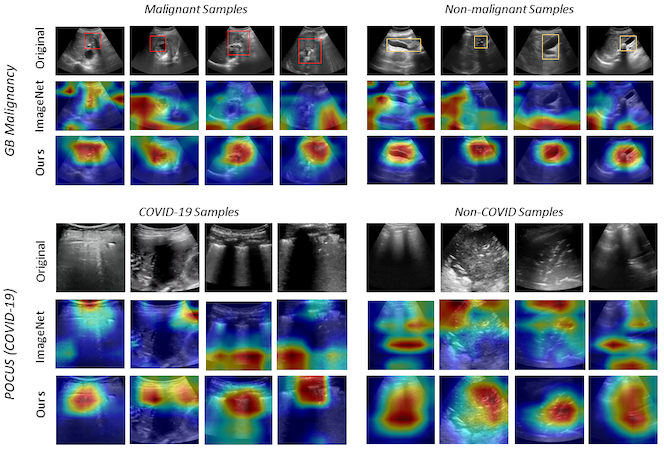
\includegraphics[width=\linewidth]{figs/usucl/cam-view.png}
    \caption[Grad-CAM visuals of the models with ImageNet pretraining and our contrastive pretraining]{Grad-CAM visuals of the last convolution layer in ImageNet pretrained model and the model pretrained using our method. The attention regions of contrastive backbones are more precise and clinically relevant.}
    \label{usucl_fig:cam_view}
\end{figure}

\begin{table}[t]
	\centering
    \footnotesize
	\setlength{\tabcolsep}{10pt}
	%\resizebox{ \linewidth}{!}{%
	\begin{tabular}{ccccc}
		\toprule
		\multicolumn{2}{c}{\textbf{Type of negative used}}& \multirow{2}{*}{\textbf{Acc.}} & \multirow{2}{*}{\textbf{Spec.}} & \multirow{2}{*}{\textbf{Sens.}} \\
		Cross-video & Intra-video & & & \\
		\midrule
		 \checkmark & & 0.890 $\pm$ 0.062 & 0.897 $\pm$ 0.061 & 0.869 $\pm$ 0.108 \\
		 & \checkmark & 0.893 $\pm$ 0.057 & 0.904 $\pm$ 0.059 & 0.835 $\pm$ 0.109 \\
		 \checkmark & \checkmark & 0.921 $\pm$ 0.034 & 0.926 $\pm$ 0.043 & 0.900 $\pm$ 0.046 \\
		\bottomrule
	\end{tabular}
	%}
    \caption[Quantitative validation of joint mining of intra, and cross video negative]{Significance of joint mining of intra, and cross video negatives. While the individual mining techniques match SOTA performance in GB malignancy, pretraining with proposed joint mining  surpasses the current SOTA.}
	\label{usucl_tab:ablation_intra_loss}
\end{table}
%
\subsection{Experimental Setup}
%
We use a machine with Intel Xeon Gold 5218@2.30GHz processor and 4 Nvidia Tesla V100 GPUs for our experiments. We pretrain a ResNet50 encoder using SGD with learning rate 0.003, weight decay $10^{-4}$, and momentum 0.9 for 60 epochs. We use a batch size of 32. We employ a grid-search strategy to select the sampling hyper-parameters. We use a cosine annealing decay of the learning rate. The parameters of the anchor and positive encoders are updated using momentum contrast with momentum coefficient, $m\!=\!0.999$. The size of the queue for cross-video negative set is $|N|\!=\!96$ for GBUSV videos. For Butterfly, we use $|N|\!=\!66$. The number of intra-video negatives, $k$, was 3 for both datasets. The number of top cross-video negatives, $n$, was 4 and 2 for GBUSV and Butterfly, respectively. We fine-tune for 30 epochs with a batch size of 64. We use an SGD optimizer with learning rate 0.003, momentum 0.9, and weight decay $5\!\cdot\!10^{-4}$. Similar to the pretraining phase, we use a cosine annealing-based learning rate scheduler. 

\subsection{Comparison with Baselines}
%
We compare the ResNet50 \cite{resnet} backbone pretrained on our contrastive learning framework with ImageNet pretraining, SOTA UCL techniques SimCLR \cite{simclr}, SimSiam \cite{simsiam}, MoCo \cite{moco}, BYOL \cite{byol}, and SOTA image representation learning from video methods: Cycle-Contrast \cite{cyclecontrast} and USCL \cite{uscl}. USCL is specialized for pretraining on the USG datasets. We note the performance of our pretraining framework for the GB malignancy classification task in \cref{usucl_tab:key_results}. Our method gives 92.1\% overall accuracy which is 2 points higher than SOTA and 90\% accuracy on malignant samples (sensitivity) which is 7 points higher than USCL. Our method also outperforms human experts significantly for detecting GB malignancy from USG images (\cref{usucl_tab:perf_human}). We show the performance comparison on the POCUS dataset in \cref{usucl_tab:pocus} and observe that our method surpasses the SOTA USCL pretraining by 1.5 points. \cref{usucl_fig:cam_view} shows the Grad-CAM \cite{gradcam} visuals of the last convolution layer to demonstrate that the attention regions of contrastive backbones are more precise and clinically relevant.

% \subsubsection{Qualitative Analysis}
% %
% \cref{usucl_fig:cam_view} shows the Grad-CAM visuals using the features generated by the last convolutional layer. As compared to the ImageNet pretrained method, the attention regions of the contrastive pretrained models are far more localized. The qualitative analysis reinforces  


\subsection{Generality of our Method Across Datasets} 
%
We have shown our method's efficacy on two different tasks - (1) GB malignancy detection from abdominal USG and (2) COVID-19 detection from lung USG, which establishes the generality of our method on USG modality. We also performed preliminary analysis on the performance of a ResNet50 classifier in detecting COVID-19 from a public CT dataset \cite{cov-finetune}. We pretrained the model on another CT dataset \cite{cov-pretrain}. The (accuracy, specificity, sensitivity) for our method was (0.80, 0.81, 0.80) as compared to (0.73, 0.72, 0.74) of ImageNet pretraining, and (0.78, 0.81, 0.76) of USCL. The results are indicative of the applicability of our method across modalities. 

\subsection{Ablation Study}
%We report the ablations on the GB malignancy classification task.
\mypara{Significance of Mining Intra-Video Hard Negatives}
%
In \cref{usucl_tab:ablation_intra_loss} we observe that when the intra-video negatives are not used, the performance of malignancy detection of our method becomes comparable to that of Cycle-Contrast and USCL; both methods use only cross-video negatives. Using only cross-video negatives yields performance similar to MoCo, which is expected since our framework is built on MoCo. The current SOTA MoCo uses only cross-video negatives. On the other hand, if only intra-video negatives are used, the model performance becomes similar to that of the SOTA image contrastive techniques. This shows the importance of mining both intra-video and cross-video negatives in achieving the performance boost.


\begin{table}[t]
	\centering
    \footnotesize
	\setlength{\tabcolsep}{10pt}
	\begin{tabular}{lccc}
		\toprule
		\textbf{Method}	& \textbf{Acc.} & \textbf{Spec.} & \textbf{Sens.} \\
		\midrule
		Proposed curriculum & 0.921 $\pm$ 0.034 & 0.926 $\pm$ 0.043 & 0.900 $\pm$ 0.046 \\
		Anti-curriculum & 0.887 $\pm$ 0.064 & 0.902 $\pm$ 0.056 & 0.836 $\pm$ 0.097 \\
		Control-curriculum & 0.897 $\pm$ 0.067 & 0.918 $\pm$ 0.062 & 0.810 $\pm$ 0.114 \\
		\bottomrule
	\end{tabular}
    \caption[Effectiveness of the curriculum-based negative mining]{Effectiveness of our curriculum-based negative mining. The other alternative, curricula based trained models, lag significantly in GB malignancy classification.}
	\label{usucl_tab:ablation_curriculum}
\end{table}


\begin{table}[t]
%    \parbox{\linewidth}{
    	\centering
        \footnotesize
    	\setlength{\tabcolsep}{10pt}
        %\resizebox{ \linewidth}{!}{%
    	\begin{tabular}{llccc}
    		\toprule
    		\textbf{Backbone} & \textbf{Method}	& \textbf{Acc.} & \textbf{Spec.} & \textbf{Sens.} \\
    		\midrule
    		%
    		\multirow{3}{*}{Resnet-18} & Pretrained on \cite{imagenet} &  0.844 $\pm$ 0.053 & 0.856 $\pm$ 0.054 & 0.795 $\pm$ 0.097 \\
    		%
    		& USCL \cite{uscl} & 0.896 $\pm$ 0.061 & 0.916 $\pm$ 0.066 & 0.833 $\pm$ 0.099 \\
    		%
    		\cmidrule{2-5}%[1.5pt]
    		& Ours & 0.907 $\pm$ 0.064 & 0.919 $\pm$ 0.072 & 0.862 $\pm$ 0.069 \\
            \midrule
            \multirow{3}{*}{MS-SoP} & Pretrained on \cite{imagenet} &   0.882 $\pm$ 0.041 & 0.872 $\pm$ 0.034 & 0.889 $\pm$ 0.055 \\
    		%
    		& USCL \cite{uscl} & 0.892 $\pm$ 0.072 & 0.903 $\pm$ 0.052 & 0.853 $\pm$ 0.091 \\
    		%
    		\cmidrule{2-5}%[1.5pt]
    		& Ours & 0.913 $\pm$ 0.042 & 0.915 $\pm$ 0.044 & 0.914 $\pm$ 0.081 \\
    		\bottomrule
    	\end{tabular}
    	%}
        \caption[Performance of different backbones with our contrastive framework]{Finetuning performance of ResNet18 and MS-SoP (refer \cref{chap:gbcnet}) for classifying GBC from USG images. All models, namely, ResNet50, ResNet18, and MS-SoP backbones show better accuracy and sensitivity of GB malignancy detection with contrastive pretraining as compared to the ImageNet pretraining or the previous SOTA \cite{uscl}.}
    	\label{usucl_tab:res18_gbc_results}
\end{table}

\mypara{Effectiveness of Curriculum-based Negative Mining}
%
We propose to use increasing order of hardness for negative mining during the training. To assert the effectiveness of such a curriculum, we compare the curriculum with two possible alternatives - (i) \emph{anti-curriculum} initially trains with harder negatives and progressively lowers the hardness of the negatives, and (ii) \emph{control-curriculum}  does not order the negatives according to their hardness. We initially train the model with temporally close intra-video negatives during the anti-curriculum and gradually start sampling temporally distant negatives. During the last few epochs, only the cross-video negatives are used. \cref{usucl_tab:ablation_curriculum} shows the performance comparison of the proposed hardness-sensitive curriculum over the two alternative curricula.

\mypara{Performance with Other Backbones}
%
We compare the fine-tuning performance of ResNet18 and our own MS-SoP \cite{basu2022surpassing} backbones pretrained using the proposed contrastive method, with the ImageNet-pretrained and USCL-pretrained backbones. We show the results in \cref{usucl_tab:res18_gbc_results}. The superior performance of various backbones pretrained with our method indicates the generalizability of our framework to multiple backbones.

\mypara{Sensitivity of Hyper-parameters}
%
\cref{usucl_fig:sens-hyper} shows the sensitivity of three important pretraining hyper-parameters on the accuracy of the downstream tasks for our method. We conduct tuning of the following hyper-parameters -- (1) number of intra-video negatives ($k$), (2) number of top cross-video negatives ($n$), and (3) the queue size ($|N|$).
%
\begin{figure}[t]
    \centering
    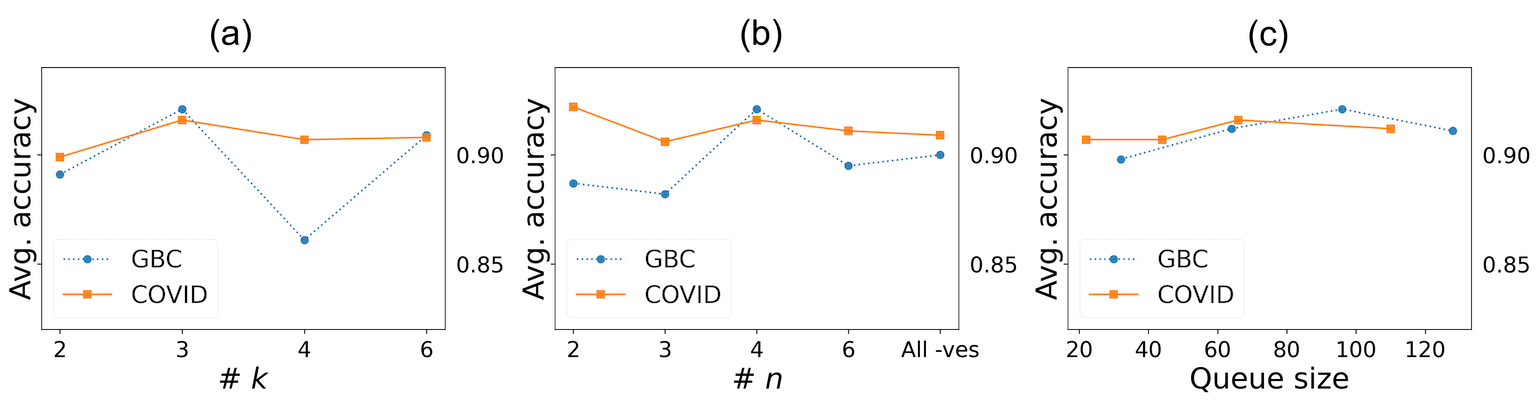
\includegraphics[width=\linewidth]{figs/usucl/sensitivity.png}
    \caption[Sensitivity of pretraining hyper-parameters]{Sensitivity of pretraining hyper-parameters - (a) number of intra-video negatives ($k$), (b) number of top cross-video negatives ($n$), and (c) queue size ($|N|$) - on downstream accuracy. Mean cross-val accuracy is shown for GB Cancer and COVID.}
    \label{usucl_fig:sens-hyper}
\end{figure}

\section{Conclusion}
%
GBC poses a formidable challenge for the off-the-shelf deep classifiers due to the low inter-class variance and high intra-class variability of malignant regions in USG images. On the other hand, the need of costly bounding box annotations of pathological regions limits the practical applicability of object detectors in SOTA frameworks such as GBCNet. 

In this chapter, we mitigate the reliance on additional labelling and explore learning with limited supervised data. We introduce a robust unsupervised contrastive learning framework tailored to address the crucial challenge of learning with limited supervised data in the realm of GBC detection from USG images. Our innovative framework leverages the unlabelled USG videos, and strategically incorporates both intra-video and cross-video negatives through a hardness-aware curriculum. The method demonstrates superior performance compared to human experts, ImageNet-pretrained DNNs, and DNNs pretrained with SOTA contrastive pretraining methods specifically designed for the USG modality.

%In this chapter, we mitigate the reliance on additional labelling and explore two different routes to learn with limited supervised data. \textbf{(1)} First, we introduce a robust unsupervised contrastive learning framework tailored to address the crucial challenge of learning with limited supervised data in the realm of GBC detection from USG images. Our innovative framework leverages the unlabelled USG videos, and strategically incorporates both intra-video and cross-video negatives through a hardness-aware curriculum. The method demonstrates superior performance compared to human experts, ImageNet-pretrained DNNs, and DNNs pretrained with SOTA contrastive pretraining methods specifically designed for the USG modality.

%%% ---- PART 2 ---- %%
\chapter{Learning from Limited Supervised Data II: Weakly Supervised GBC Detection}
\label{chap:wsod}
Earlier, in \Cref{chap:limited}, we discussed the usage of unlabelled video data in an unsupervised contrastive framework to learn downstream representation for GBC detection. Unlike GBCNet, our design did not require the costly bounding box annotations.
In this chapter, we explore another direction towards learning from limited supervised data -- using a weakly supervised object detection technique to detect GBC with only image-level labels instead of the costly bounding box annotations during training. Unlike the earlier design in \Cref{chap:limited} , we do not require any additional video data.

%the  We investigate two distinct approaches towards this direction -- (1) we introduce an unsupervised contrastive framework designed to leverage unlabelled video data for effective representation learning, ultimately benefiting downstream GBC detection from USG images, and (2) we use a weakly supervised object detection technique to detect GBC with only image-level labels instead of the costly bounding box annotations during training.
This chapter is based on the following published work:
\par \noindent [1] \textit{Soumen Basu, Ashish Papanai, Mayank Gupta, Pankaj Gupta, and Chetan Arora.``Gall Bladder Cancer Detection from US Images with only Image Level Labels.'' International Conference on Medical Image Computing and Computer-Assisted Intervention (MICCAI). 2023}.
%\label{chap:limited}

%\section{Weakly Supervised GBC Detection}
%
%Automated detection of Gallbladder Cancer (GBC) from Ultrasound (USG) images is an important problem, which has drawn increased interest from researchers. However, most of these works use difficult-to-acquire information such as bounding box annotations or additional USG videos. In this paper, we focus on GBC detection using only image-level labels. Such annotation is usually available based on the diagnostic report of a patient, and do not require additional annotation effort from the physicians.  We posit that even when we have only the image level label, still formulating the problem as object detection (with bounding box output) helps a deep neural network (DNN) model focus on the relevant region of interest. Since no bounding box annotations is available for training, we pose the problem as weakly supervised object detection (WSOD). Motivated by the recent success of transformer models in object detection, we train one such model, DETR, using multi-instance-learning (MIL) with self-supervised instance selection to suit the WSOD task. Our proposed method demonstrates an improvement of AP and detection sensitivity over the SOTA transformer-based and CNN-based WSOD methods. Project page is at \url{https://gbc-iitd.github.io/wsod-gbc}.
 
% \keywords{Weakly Supervised Object Detection \and Ultrasound \and Gallbladder Cancer}
% \end{abstract}

% \begin{figure}[t]
%     \centering
%     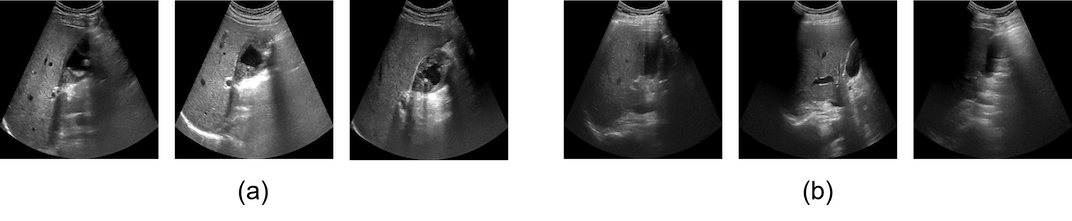
\includegraphics[width=0.9\linewidth]{figs/wsod/teaser.png}
%     \caption[Visualization of low inter-class and high intra-class variability]{(a) Low inter-class variability. The first two GBs show benign wall thickening, and the third one shows malignant thickening. However, the appearance of the GB in all three images is very similar. (b) High intra-class variability. All three images have been scanned from the same patient, but due to the sensor's scanning plane, the appearances change drastically.}
%     \label{wsod_fig:teaser}
% \end{figure}

%
% ---- Introduction ----
%
\section{Introduction}
%
%\gbc is a deadly disease that is difficult to detect at an early stage \cite{howlader2017seer,gupta2021locally}. Early diagnosis can significantly improve the survival rate \cite{hong2014surgical}. Non-ionizing radiation, low cost, and accessibility make \usg a popular non-invasive diagnostic modality for patients with suspected gall bladder (\gb) afflictions. However, identifying signs of \gbc from routine \usg imaging is challenging for radiologists \cite{gupta2020imaging}. In recent years, automated \gbc detection from \usg images has drawn increased interest \cite{basu2022surpassing,basu2022unsupervised} due to its potential for improving diagnosis and treatment outcomes. Many of these works formulate the problem as an object detection, since training a image classification model for \gbc detection seems challenging due to the reasons outlined in the abstract (also see \cref{wsod_fig:teaser}).

Earlier, we have developed \gbcnet \cite{basu2022surpassing}, a \cnn-based model, to achieve the \sota performance on classifying malignant \gb from \usg images. \gbcnet uses a two-stage pipeline consisting of object detection followed by classification, and requires bounding box annotations for \gb and malignant regions (region of interest or ROI) for training the detection part. Such bounding box annotations surrounding the pathological regions are time-consuming and require an expert radiologist for annotation. This makes it expensive and non-viable for curating large datasets for training large \dnn models. We have also exploited additional unlabeled video data earlier for learning good representations for downstream \gbc classification and obtained performance comparable to \gbcnet using a ResNet50 \cite{resnet} classifier. The reliance of both \sota techniques on additional annotations or data, limits their applicability in clinical setup. At times, the information such as bounding box annotations or additional USG videos can become difficult to acquire. On the other hand, the image-level malignancy label is usually available at a low cost, as it can be obtained readily from the diagnostic report of a patient without additional effort from clinicians. 

We have seen previously that the off-the-shelf DNN-based classifiers do not perform well in case of detecting GBC from USG image. %Our analysis revealed that it is difficult to train the standard image classification models for GBC detection due to the presence of artifacts including shadows or textures. 
Additionally, the low inter-class variance (a malignant region usually occupies only a small portion of a USG image), high intra-class variance (due to the USG sensor capturing a 2D slice of a 3D object leading to large viewpoint variations), and low training data availability add to the difficulties. Instead of training a classification pipeline, we propose to solve an object detection problem, which involves predicting a bounding box for the malignancy. The motivation is that, running a classifier on a focused attention/ proposal region in an object detection pipeline would help tackle the low inter-class and high intra-class variations. In fact, \gbcnet also follows the same principle of running classifiers on focused regions (ROI). However, since we only have image-level labels available in the current setup, we formulate the problem as a Weakly Supervised Object Detection (\wsod) problem. 

As transformers are increasingly outshining \cnns due to their ability to aggregate focused cues from a large area \cite{vit,detr}, we choose to use transformers in our model. However, in our initial experiments \sota \wsod methods for transformers failed miserably. These methods primarily rely on training a classification pipeline and later generating activation heatmaps using attention and drawing a bounding box circumscribing the heatmaps \cite{tscam,scm} to show localization. %However, for \gbc detection, this line of work was not helpful as we discussed earlier. 

Inspired by the success of the Multiple Instance Learning (\mil) paradigm for weakly supervised training on medical imaging tasks \cite{transmil,swinmil}, we train a detection transformer, \detr, using the \mil paradigm for weakly supervised malignant region detection. In this, one generates region proposals for images, and then considers the images as bags and region proposals as instances to solve the instance classification (object detection) under the \mil constraints \cite{dietterich1997solving}. At inference, we use the predicted instance labels to predict the bag labels. Our experiments affirm the effectiveness of employing WSOD in circumventing the challenges posed by the limited availability of densely annotated data (bounding box annotations) in USG images. Our approach proves successful in detecting and localizing GBC from USG images using only image-level labels. We also provide a strong baseline for weakly supervised \gbc detection and localization in \usg images, which has not been tackled earlier. In addition, we assess the generality of the proposed weakly supervised DETR model on detecting polyps from colonoscopy images.

%Our experiments validate the utility of this approach of using weakly supervised object detection in circumventing the densely annotated data availability challenges in \usg images and detecting \gbc accurately from \usg images using only image-level labels.

% \mypara{Contributions} The key contributions of this work are:
% \begin{itemize}%[label=\textbf{(\arabic*)}]
% \itemsep0em
% 	\item  We design a novel \detr variant based on \mil with self-supervised instance learning towards the weakly supervised disease detection and localization task in medical images. Although \mil and self-supervised instance learning has been used for \cnns \cite{oicr}, such a pipeline has not been used for transformer-based detection models.  
% 	%
%     \item We formulate the \gbc classification problem as a weakly supervised object detection problem to mitigate the effect of low inter-class and large intra-class variances, and solve the difficult \gbc detection problem on \usg images without using the costly and difficult to obtain additional annotation (bounding box) or video data.
%     %
% 	\item Our method provides a strong baseline for weakly supervised \gbc detection and localization in \usg images, which has not been tackled earlier. %
% \end{itemize}

%
% ---- Dataset ----
%
\begin{figure}[t]
    \centering
    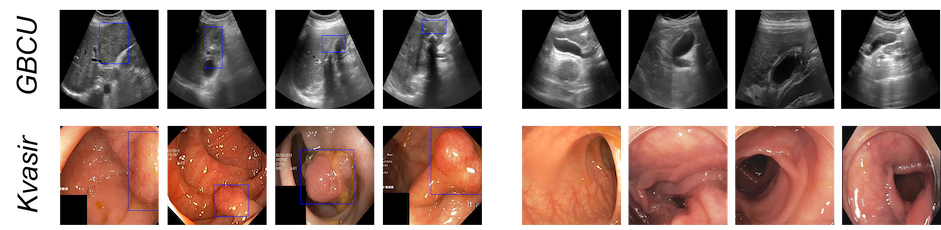
\includegraphics[width=\textwidth]{figs/wsod/data_sample.png}
    \caption[Visuals of GBC and Polyp data samples]{Samples from the GBCU \cite{basu2022surpassing} and Kvasir-SEG \cite{kvasir} datasets. Four samples from each disease and non-disease classes are shown on the left and right, respectively. Disease locations are shown by bounding boxes (blue colored).}
    \label{wsod_fig:data_sample}
\end{figure}

\section{Data}

\subsection{GBC Detection in USG Images}
%
We use our GBCU dataset \cref{data:gbcu} consisting of 1255 image samples from 218 patients. The dataset contains 990 non-malignant (171 patients) and 265 malignant (47 patients) \gb images. Recall that GBCU contains image labels as well as bounding box annotations showing the malignant regions. Note that, we use only the image labels for training the weakly supervised object detectors. We report results on 5-fold cross-validation. We did the cross-validation splits at the patient level, and all images of any patient appeared either in the train or validation split. 

\subsection{Polyp Detection in Colonoscopy Images}
%
We use the publicly available Kvasir-SEG \cite{kvasir} dataset consisting of 1000 white light colonoscopy images showing polyps (c.f. \cref{wsod_fig:data_sample}). Since Kvasir-SEG does not contain any control images, we add 600 non-polyp images randomly sampled from the PolypGen \cite{polypgen} dataset. Since the patient information is not available with the data, we use random stratified splitting for 5-fold cross-validation.

%
% ---- Methods ----
%
\section{Our Method}

\begin{figure}[t]
    \centering
    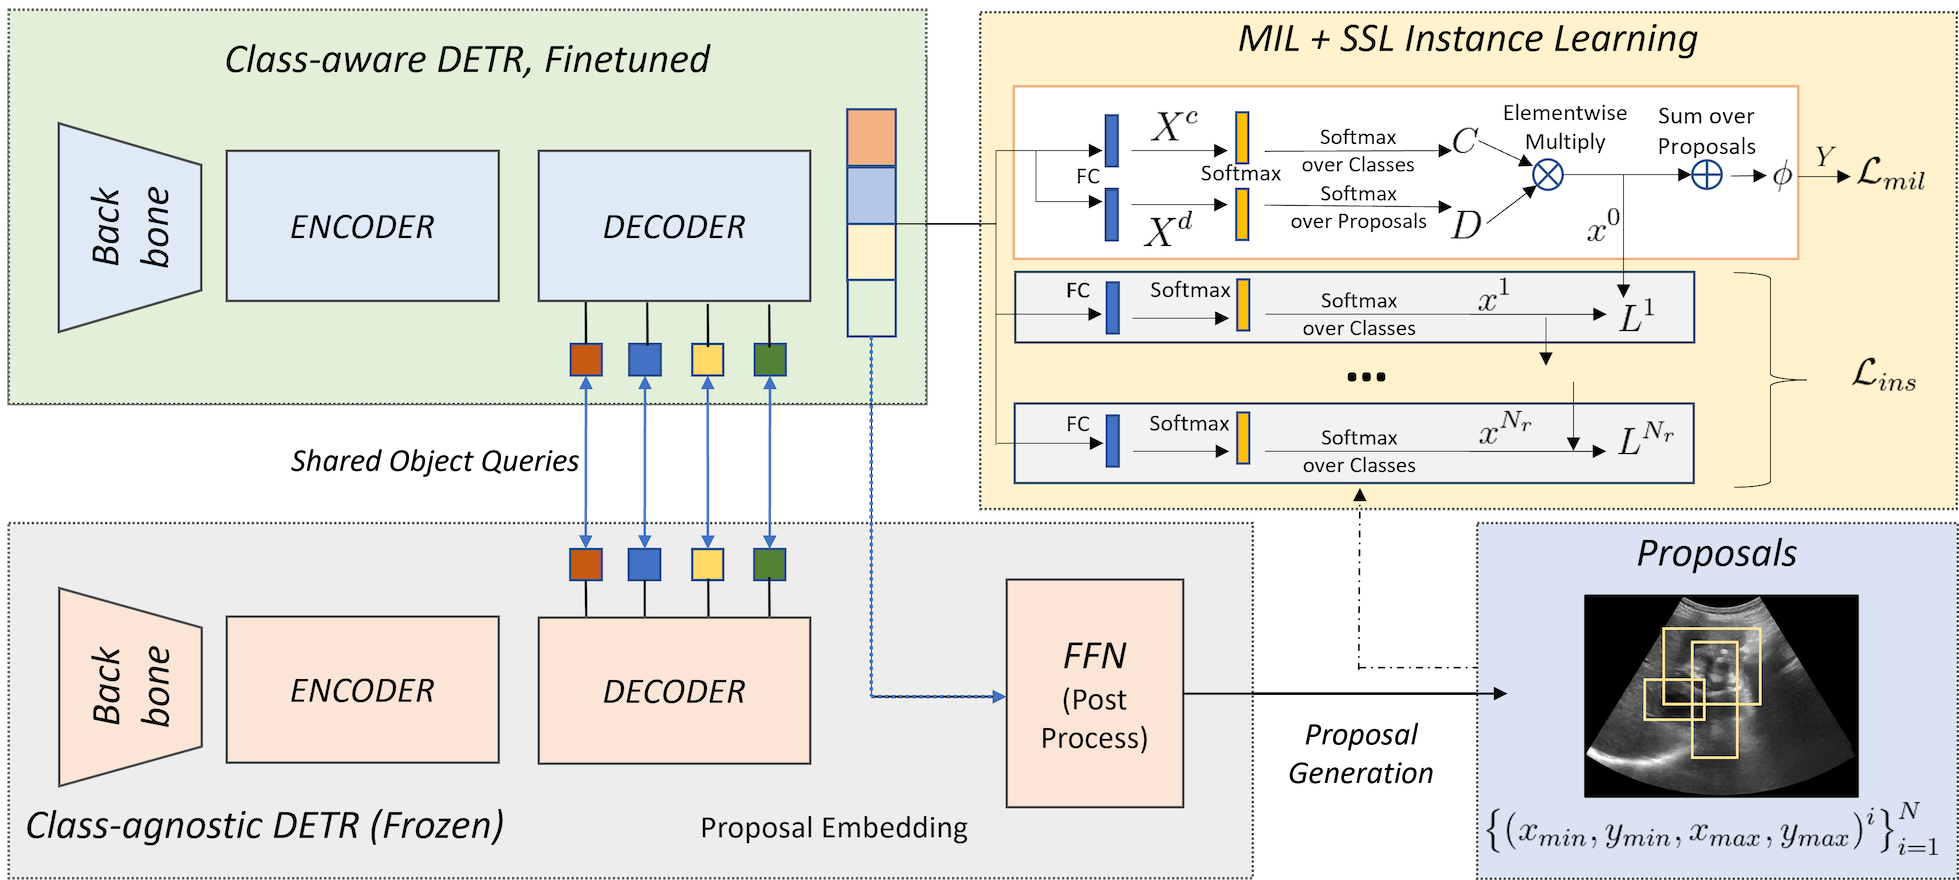
\includegraphics[width=0.9\linewidth]{figs/wsod/arch.png}
    \caption[Overview of the proposed Weakly Supervised \detr architecture]{Overview of the proposed Weakly Supervised \detr architecture. The location information in the object queries learned by the class-agnostic \detr ensures generation of high-quality proposals. The \mil framework uses the proposal embeddings generated at the class-aware branch. }
    \label{wsod_fig:method}
\end{figure}

\mypara{Revisiting \detr}
%
The \detr \cite{detr} architecture utilizes a \texttt{ResNet} \cite{resnet} backbone to extract \texttt{2D} convolutional features, which are then flattened and added with a positional encoding, and fed to the self-attention-based transformer encoder. The decoder uses cross-attention between learned object queries containing positional embedding, and encoder output to produce output embedding containing the class and localization information. The number of object queries, and the decoder output embeddings is set to 100 in \detr. Subsequently, a feed-forward network generates predictions for object bounding boxes with their corresponding labels and confidence scores. 

\mypara{Model Architecture}
%
\cref{wsod_fig:method} gives an overview of our method. We use a \texttt{COCO} pre-trained class-agnostic \detr as proposal generator. The learned object queries contain the embedded positional information of the proposal. Class-agnostic indicates that all object categories are considered as a single object class, as we are only interested in the object proposals. We then finetune a regular, class-aware \detr for the \wsod task. This class-aware \detr is initialized with the checkpoint of the class-agnostic \detr. The learned object queries from the class-agnostic \detr is frozen and shared with the \wsod \detr during finetuning to ensure that the class-aware \detr attends similar locations of the object proposals. The class-agnostic \detr branch is frozen during the finetuning phase. We finally use the \mil-based instance classification with the self-supervised instance learning over the finetuning branch. For \gbc classification, if the model generates bounding boxes for the input image, then we predict the image to be malignant, since the only object present in the data is the cancer. 

\mypara{\mil Setup}
%
The decoder of the fine-tuning \detr generates $R$ $d$-dimensional output embeddings. Each embedding corresponds to a proposal generated by the class-agnostic \detr. We pass these embeddings as input to two branches with \texttt{FC} layers to obtain the matrices $X^c \in \mathbb{R}^{R\times N_c}$ and $X^r \in \mathbb{R}^{R\times N_c}$, where $R$ is the number of object queries (same as proposals) and $N_c$ is the number of object (disease) categories. Let $\sigma(\cdot)$ denote the softmax operation. 
We then generate the class-wise and detection-wise softmax matrices $C\in\mathbb{R}^{R\times N_c}$ and $D\in\mathbb{R}^{R\times N_c}$, where $C_{ij} = \sigma((X^c)^T_j)i$ and $D_{ij} = \sigma(X^r_i)j$, and $X_i$ denotes the $i$-th row of $X$. $C$ provides classification probabilities of each proposal, and $D$ provides the relative score of the proposals corresponding to each class. The two matrices are element-wise multiplied and summed over the proposal dimension to generate the image-level classification predictions, $\phi\in\mathbb{R}^{N_c}$: 
\begin{align}
\phi_j = \sum_{i=1}^R C_{ij}\cdot D_{ij}
\end{align}
%
Notice, $\phi_j \in (0,1)$ since $C_{ij}$ and $D_{ij}$ are normalized. Finally, the negative log-likelihood loss between the predicted labels, and image labels $y\in\mathbb{R}^{N_c}$ is computed as the \mil loss:
%
\begin{align}
\mathcal{L}_\text{mil} = -\sum_{i=1}^{N_c}[{y_i \log{\phi_i}} + (1-y_i) \log{(1-\phi_i)}]   
\end{align}
The \mil classifier further suffers from overfitting to the distinctive classification features due to the mismatch of classification and detection probabilities \cite{oicr}. To tackle this, we further use a self-supervised module to improve the instances.

\mypara{Self-supervised Instance Learning}
% 
Inspired by \cite{oicr}, we design a instance learning module with $N_r$ blocks in a self-supervised framework to refine the instance scores with instance-level supervision. Each block consists of an \texttt{FC} layer. A class-wise softmax is used to generate instance scores $x^n \in \mathbb{R}^{R\times(N_c+1)}$ at $n$-th block. $N_c+1$ includes the background/ no-finding class. Instance supervision of each layer ($n$) is obtained from the scores of the previous layer ($x^{(n-1)}$). The instance supervision for the first layer is obtained from the \mil head. Suppose $\hat{y}^n \in \mathbb{R}^{R\times(N_c+1)}$ is the pseudo-labels of the instances. An instance ($p_j$) is labelled 1 if it overlaps with the highest-scoring instance by a chosen threshold. Otherwise, the instance is labeled $0$ as defined in \cref{eqn:inst_sample}:
\begin{align}
    m^n_j = \argmax_{i}{x^{(n-1)}_{ij}} ~;
    \qquad
    \hat{y}^n_{ij} =  
    \begin{cases}
    1, & IoU(p_j, p_{m^n_j}) \geq \tau\\
    0, & \text{otherwise}
    \end{cases}
    \label{eqn:inst_sample}
\end{align}
The loss over the instances is given by \cref{eqn:inst_loss}:
\begin{align}
    \mathcal{L}_{ins} = - \frac{1}{N_r} \sum_{n=1}^{N_r} \frac{1}{R} \sum_{i=1}^R \sum_{j=1}^{N_c+1} w^{n}_{i} \hat{y}^{n}_{ij} \log x^n_{ij}
    \label{eqn:inst_loss}
\end{align}
Here $x^n_{ij}$ denotes the score of $i$-th instance for $j$-th class at layer $n$. Following \cite{oicr}, the loss weight $w^n_{i} = x^{(n-1)}_{i\,m^n_j}$ is applied to stabilize the loss.
Assuming $\lambda$ to be a scaling value, the overall loss function is given in \cref{eqn:loss}:
\begin{align}
    \mathcal{L} = \mathcal{L}_{mil} + \lambda\mathcal{L}_{ins} 
    \label{eqn:loss}
\end{align}

%
% ---- Experiments and Results ----
%
\section{Experiments and Results}
%
\subsection{Experimental Setup}
%
We use a machine with Intel Xeon Gold 5218@2.30GHz processor and 8 Nvidia Tesla V100 GPUs for our experiments. The model is trained using SGD with LR 0.001 (for MIL head), weight decay $10^{-6}$, and momentum 0.9 for 100 epochs with batch size 32. The LR at backbone and transformer are 0.003, and 0.0003, respectively. We use a cosine annealing of the LR. 

%
\begin{table}[t]
	\centering
    \footnotesize
	\setlength{\tabcolsep}{10pt}
    %\resizebox{ \linewidth}{!}{%
	\begin{tabular}{llcc}
		\toprule
		\multirow{2}{*}{\textbf{Method}} & \multirow{2}{*}{\textbf{Venue (year)}} & \textbf{GBC} & \textbf{Polyp} \\ 
        & & $AP_{25}$ & $AP_{25}$ \\
        \midrule
        TS-CAM \cite{tscam} & ICCV (2021) & 0.024 $\pm$ 0.008 & 0.058 $\pm$ 0.015 \\
        SCM \cite{scm} & ECCV (2022) & 0.013 $\pm$ 0.001 & 0.082 $\pm$ 0.036 \\
        OD-WSCL \cite{odwscl} & ECCV (2022) & 0.482 $\pm$ 0.067 & 0.239 $\pm$ 0.032 \\
        WS-DETR \cite{wsdetr} & WACV (2023) & 0.520 $\pm$ 0.088 & 0.246 $\pm$ 0.023 \\
        Point-Beyond-Class \cite{pointdetr} & MICCAI (2022) & 0.531 $\pm$ 0.070 & 0.283 $\pm$ 0.022 \\
        \midrule
        Ours & MICCAI (2023) & 0.628 $\pm$ 0.080 & 0.363 $\pm$ 0.052 \\
        \bottomrule
    \end{tabular}
    %}
    \caption[Weakly supervised disease detection performance of SOTA and our method]{Weakly supervised disease detection performance comparison of our method and SOTA baselines in GBC and Polyps. We report Average Precision at IoU 0.25 ($AP_{25}$).}
    \label{wsod_tab:wsod}
\end{table}

%
\begin{figure}[t]
    \centering
    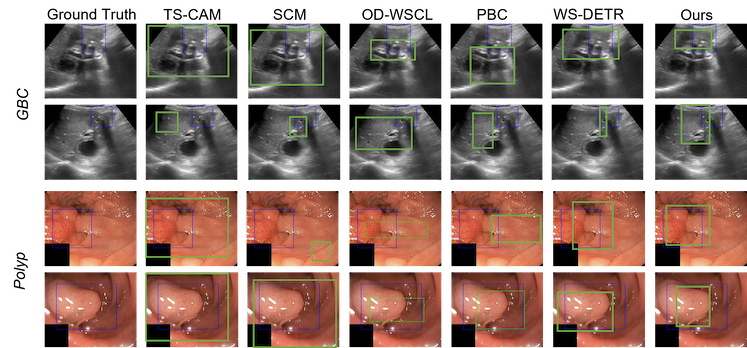
\includegraphics[width=\linewidth]{figs/wsod/visual.png}
    \caption[Qualitative analysis of the predicted bounding boxes]{Qualitative analysis of the predicted bounding boxes. Ground truths are in blue, and predictions are in green. We compare with \sota \wsod techniques and our proposed method. Our method predicts much tighter bounding boxes that cover the clinically significant disease regions.}
    \label{wsod_fig:visuals}
\end{figure}

\subsection{Comparison with Baseline WSOD Methods}
%
\cref{wsod_tab:wsod} shows the bounding box localization results of the \wsod task. Our method surpasses all latest \sota \wsod techniques by 9 points, and establishes itself as a strong \wsod baseline for \gbc localization in \usg images. Our method also achieves 7-point higher AP score for polyp detection. We present visualizations of the predicted bounding boxes in \cref{wsod_fig:visuals} which shows that the localization by our method is more precise and clinically relevant as compared to the baselines. 
%
\begin{table}[t]
	\centering
    \footnotesize
	\setlength{\tabcolsep}{6pt}
%	\resizebox{ \linewidth}{!}{%
	\begin{tabular}{lcccc}
		\toprule
        \multirow{2}{*}{\textbf{Design}} & \multicolumn{2}{c}{\textbf{GBC}} & \multicolumn{2}{c}{\textbf{Polyp}} \\
		 & \textbf{$AP_{25}$} & \textbf{Sens.} & \textbf{$AP_{25}$} & \textbf{Sens.} \\
		\midrule
            MIL + DETR & 0.520 $\pm$ 0.088 & 0.833 $\pm$ 0.034 & 0.246 $\pm$ 0.023 & 0.882 $\pm$ 0.034\\	        
            MIL + SSL + DETR (Ours) & 0.628 $\pm$ 0.080 & 0.861 $\pm$ 0.089 & 0.363 $\pm$ 0.052 & 0.932 $\pm$ 0.022\\
		\bottomrule
	\end{tabular}
%	}
    \caption[Ablation study on the proposed weakly supervised DETR]{Ablation study. Performance of \mil-framework variants on \detr. We compare the AP and detection sensitivity.} 
	\label{wsod_tab:ablation}
\end{table}

\begin{table}[t]
	\centering
    \footnotesize
    \setlength{\tabcolsep}{6pt}
	%\resizebox{ \linewidth}{!}{%
	\begin{tabular}{llccc}
		\toprule
		{\textbf{Type}} & {\textbf{Method}} & {\textbf{Acc.}} &  {\textbf{Spec.}} & {\textbf{Sens.}} \\
		\midrule
		%
		\multirow{2}{*}{CNN Classifier} 
		& ResNet50 \cite{resnet} & 0.867 $\pm$ 0.031 & 0.926 $\pm$ 0.069 & 0.672 $\pm$ 0.147  \\
		%
        & Inception V3 & 0.844 $\pm$ 0.039 & 0.953 $\pm$ 0.029 & 0.807 $\pm$ 0.097 \\
		%& InceptionV3 \cite{inception} & 0.869 $\pm$ 0.039 & 0.913 $\pm$ 0.032 & 0.708 $\pm$ 0.078 \\
  		%
        \midrule
        \multirow{4}{*}{Transformer Classifier} 
        & ViT \cite{vit} & 0.803 $\pm$ 0.078 & 0.901 $\pm$ 0.050 & 0.860 $\pm$ 0.068  \\
		%
		& DEIT \cite{touvron2021training} & 0.829 $\pm$ 0.030 & 0.900 $\pm$ 0.040 & 0.875 $\pm$ 0.063 \\
		%
		& PVTv2 \cite{wang2021pvtv2} & 0.824 $\pm$ 0.033 & 0.887 $\pm$ 0.057 & 0.894 $\pm$ 0.076 \\
        %& RadFormer \cite{basu2023radformer} & 0.921 $\pm$ 0.062 & 0.961 $\pm$ 0.049 & 0.923 $\pm$ 0.062  \\
		\midrule
        \multirow{4}{*}{Additional Data/ Annotation}
		& USCL \cite{uscl} & 0.889 $\pm$ 0.047 & 0.895 $\pm$ 0.054 & 0.869 $\pm$ 0.097 \\
		%
        & US-UCL \cite{basu2022unsupervised} & 0.920 $\pm$ 0.034 & 0.926 $\pm$ 0.043 & 0.900 $\pm$ 0.046  \\
		%
		& GBCNet \cite{basu2022surpassing} & 0.921 $\pm$ 0.029 & 0.967 $\pm$ 0.023 & 0.919 $\pm$ 0.063 \\
        %
        & Point-Beyond-Class \cite{pointdetr} & 0.929  $\pm$  0.013 & 0.983  $\pm$  0.042 & 0.731  $\pm$  0.077 \\
		%
        \midrule
		\multirow{4}{*}{SOTA WSOD} &
		TS-CAM \cite{tscam} & 0.862 $\pm$ 0.049 & 0.879 $\pm$ 0.049 & 0.751 $\pm$ 0.045   \\
		%
		& SCM \cite{scm} & 0.795 $\pm$ 0.101 & 0.783 $\pm$ 0.130 & 0.849 $\pm$ 0.072  \\
		%
		& OD-WSCL \cite{odwscl} & 0.815 $\pm$ 0.144 & 0.805 $\pm$ 0.129 & 0.847 $\pm$ 0.214   \\
		%
        & WS-DETR \cite{wsdetr} & 0.839 $\pm$ 0.042 & 0.843 $\pm$ 0.028 & 0.833 $\pm$ 0.034 \\
		%
		\midrule%[1.5pt]
		WSOD & Ours & 0.834 $\pm$ 0.057 & 0.817 $\pm$ 0.061 & 0.861 $\pm$ 0.089 \\
		\bottomrule
	\end{tabular}
	%}
    \caption[comparison of the proposed WSOD and other \sota methods in \gbc classification]{Performance comparison of our method and other \sota methods in \gbc classification. US-UCL refers to the unsupervised contrastive method we discussed in \cref{chap:usucl}. We report accuracy, specificity, and sensitivity for all models. }
	\label{wsod_tab:key_results}
\end{table}

% \begin{table}[t]
% 	\centering
% 	\setlength{\tabcolsep}{10pt}
% 	\caption{Comparison with \sota \wsod baselines in classifying Polyps from Colonoscopy images. }
%     \resizebox{ 0.9\linewidth}{!}{%
% 	\begin{tabular}{lccc}
% 		\toprule
% 		%\multirow{2}{*}{\textbf{Method}} & \multicolumn{2}{c}{\textbf{GBC}} & \multicolumn{2}{c}{\textbf{Polyp}} \\ 
%         \textbf{Method} & \textbf{Acc.} & \textbf{Spec.} & \textbf{Sens.}  \\
% 		\midrule
% 		%
% 		TS-CAM \cite{tscam} & 0.704 $\pm$ 0.017 & 0.394 $\pm$ 0.042 & 0.891 $\pm$ 0.054 \\
% 		%
% 		SCM \cite{scm} & 0.751 $\pm$ 0.026 & 0.523 $\pm$ 0.014 & 0.523 $\pm$ 0.016  \\
% 		%
% 		OD-WSCL\cite{odwscl} & 0.805 $\pm$ 0.056 & 0.609 $\pm$ 0.076 & 0.923 $\pm$ 0.034  \\
% 		%
% 		WS-DETR \cite{wsdetr} & 0.857 $\pm$ 0.071 & 0.812 $\pm$ 0.088 & 0.882 $\pm$ 0.034 \\
% 		%
% 		Point-Beyond-Class \cite{pointdetr} & 0.953 $\pm$ 0.007 & 0.993 $\pm$ 0.004 & 0.924 $\pm$ 0.011 \\
% 		%
% 		\midrule%[1.5pt]
% 		Ours & 0.878 $\pm$ 0.067 & 0.785 $\pm$ 0.102 & 0.932 $\pm$ 0.022 \\
% 		\bottomrule
% 	\end{tabular}
% 	}
% 	\label{wsod_tab:polyp_results}
% \end{table}

\subsection{Generality of the Method}
%
We assess the generality of our method by applying it to polyp detection on colonoscopy images. The applicability of our method on two different tasks - (1) \gbc detection from \usg and (2) Polyp detection from Colonoscopy, indicates the generality of the method across modalities. 

\subsection{Ablation Study}
%
We show the detection sensitivity to the self-supervised instance learning module in \cref{wsod_tab:ablation} for two variants, (1) vanilla \mil head on \detr, and (2) \mil with self-supervised instance learning on \detr. \cref{wsod_tab:ablation} shows the Average Precision and detection sensitivity for both diseases. The results establish the benefit of using the self-supervised instance learning. %Other ablations related to the hyper-parameter sensitivity is given in Supplementary Fig. S1.

\subsection{Classification Performance}
%
We compare our model with the standard \cnn-based and Vision Transformer-based classifiers, \sota \wsod-based classifiers, and \sota classifiers using additional data or annotations (\cref{wsod_tab:key_results}). Our method beats the \sota weakly supervised techniques and achieves 1.2\% higher sensitivity for GBC detection. The current \sota \gbc detection models require additional bounding box annotation \cite{basu2022surpassing} or, \usg videos \cite{basu2022unsupervised,uscl}. However, even without these additional bounding box annotations or data, our method reaches 86.1\% detection sensitivity. 
%The results for polyp classification are reported in \cref{wsod_tab:polyp_results}. Although our method has a slightly lower specificity, the sensitivity surpasses the baselines reported in literature \cite{jha2021real}, and the \sota \wsod based baselines. 

%
% ---- Conclusion ----
%
\section{Conclusion}
%
%GBC poses a formidable challenge for the off-the-shelf deep classifiers due to the low inter-class variance and high intra-class variability of malignant regions in USG images. On the other hand, the need of costly bounding box annotations of pathological regions limits the practical applicability of object detectors in SOTA frameworks such as GBCNet. 

%In this chapter, we mitigate the reliance on additional labelling and explore two different routes to learn with limited supervised data. \textbf{(1)} First, we introduce a robust unsupervised contrastive learning framework tailored to address the crucial challenge of learning with limited supervised data in the realm of GBC detection from USG images. Our innovative framework leverages the unlabelled USG videos, and strategically incorporates both intra-video and cross-video negatives through a hardness-aware curriculum. The method demonstrates superior performance compared to human experts, ImageNet-pretrained DNNs, and DNNs pretrained with SOTA contrastive pretraining methods specifically designed for the USG modality.
%
%While interest in automated GBC detection is on the rise, training standard image classification models for this task remains a hurdle. 
In this chapter, we explore an alternative approach to using additional unlabelled video data. We propose a weakly supervised object detection/ localization method using DETR (DEtection TRansformers) within a Multiple Instance Learning (MIL) framework. Our experiments showcase competitive performance without the need for additional annotation or data, presenting a solution to the key challenge of learning with limited data in medical image computing. This approach provides a simplified training methodology applicable in hospitals with readily available local data, ultimately enhancing the effectiveness of automated GBC detection. 


% We propose a robust Unsupervised Contrastive Learning framework that exploits both intra-video and cross-video negatives through a hardness-aware curriculum. Our framework surpasses the human experts, imageNet-pretrained DNNs, and DNNs pretrained with SOTA contrastive learning methods specialized for USG modality.

% \gbc is a difficult-to-detect disease that benefits greatly from early diagnosis. 
% While automated \gbc detection from \usg images has gained increasing interest from researchers, training a standard image classification model for this task is challenging due to the low inter-class variance and high intra-class variability of malignant regions. 
% Current \sota models for \gbc detection require costly bounding box annotation of the pathological regions, or additional \usg video data, which limit their applicability. We proposed to formulate \gbc detection as a weakly supervised object detection/ localization problem using a \detr with self-supervised instance learning in a \mil framework. Our experiments show that the approach achieves competitive performance without requiring additional annotation or data. We hope that our technique will simplify the model training at the hospitals with easily available data locally, enhancing the applicability and impact of automated \gbc detection. 


%
% ---- Bibliography ----
%
% BibTeX users should specify bibliography style 'splncs04'.
% References will then be sorted and formatted in the correct style.
%

% \section{Supplementary Material}

% %\appendix
% %\beginsupplement
% \subsubsection{Visualization of Feature Representation}
% \cref{usucl_fig:cam_view} shows the Grad-CAM visuals using the features generated by the last convolutional layer. 
% \begin{figure}[!ht]
%     \centering
%     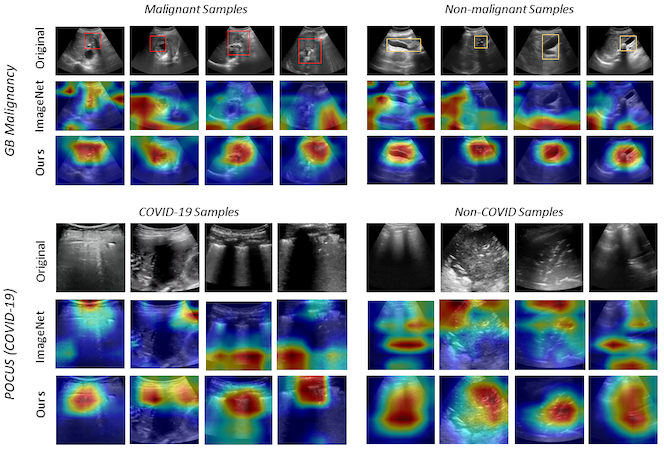
\includegraphics[width=\textwidth]{figs/usucl/cam-view.png}
%     \caption{Grad-CAM visuals of the last conv layer in ImageNet pretrained model and the model pretrained using our CL method. The attention regions of contrastive backbones are more precise and clinically relevant.}
%     \label{usucl_fig:cam_view}
% \end{figure}
%
% \subsection{Performance with Another Backbone}
% We compare the fine-tuning performance of ResNet18 backbone by pretraining with our method is compared with ImageNet-pretrained ResNet18 and USCL-pretrained ResNet18. We show the results in \cref{usucl_tab:res18_gbc_results,usucl_tab:res18_pocus_results}. In the main text, we showed performance analysis with ResNet50 backbone. The superior performance of both backbones pretrained with our method indicates the generalizability of our framework to multiple backbones.
% \begin{table}[!t]
%     \parbox{\linewidth}{
%     	\centering
%     	\setlength{\tabcolsep}{10pt}
%     	\caption{Finetuning performance of ResNet18 for classifying malignant vs. non-malignant GBs from USG images. Both ResNet50 (result in main text) and ResNet18 backbones show better accuracy and sensitivity of GB malignancy detection with contrastive pretraining as compared to the ImageNet pretraining.}
%         \resizebox{ \linewidth}{!}{%
%     	\begin{tabular}{lccc}
%     		\toprule
%     		\textbf{Method}	& \textbf{Acc.} & \textbf{Spec.} & \textbf{Sens.} \\
%     		\midrule
%     		%
%     		Pretrained on ImageNet &  0.844 $\pm$ 0.053 & 0.856 $\pm$ 0.054 & 0.795 $\pm$ 0.097 \\
%     		%
%     		USCL & 0.896 $\pm$ 0.061 & 0.916 $\pm$ 0.066 & 0.833 $\pm$ 0.099 \\
%     		%
%     		\midrule%[1.5pt]
%     		Ours & 0.907 $\pm$ 0.064 & 0.919 $\pm$ 0.072 & 0.862 $\pm$ 0.069 \\
%     		\bottomrule
%     	\end{tabular}
%     	}
%     	\label{usucl_tab:res18_gbc_results}
%     }
%     \vspace{2em}
    
%     \parbox{\linewidth}{
%         \centering
%     	\setlength{\tabcolsep}{10pt}
%     	\caption{Comparison of finetuning performance of ResNet18 using the SOTA USCL, ImageNet pretraining, and our method on POCUS. The pretraining was done on Butterfly dataset.}
%     	\resizebox{ \linewidth}{!}{%
%     	\begin{tabular}{lcccc}
%         	\toprule
%         	\multirow{2}{*}{\textbf{Method}} & \multicolumn{4}{c}{\textbf{Accuracy}} \\
%         	& \textbf{Overall} & \textbf{COVID-19} & \textbf{Pneumonia} & \textbf{Regular} \\
%         	\midrule
%         	Pretrained on ImageNet & 0.874 & 0.797 & 0.874 & 0.919  \\
%         	USCL & 0.914 & 0.916 & 0.940 & 0.906 \\
%         	\midrule
%         	Ours & 0.922 & 0.902 & 0.946 & 0.926   \\
%         	\bottomrule
%     	\end{tabular}
%     	}
%     	\label{usucl_tab:res18_pocus_results}
% 	}
% \end{table}

